% =====================================================================
\section{Phase 6: the physics-constrained generative search}\label{sec:p6}
% =====================================================================

\textbf{Goal.} Assemble everything into one honest discovery pipeline (Figure~\ref{fig:pipeline}) that searches
over candidate equations, tests each with an inverse PINN, and selects the most parsimonious supported law,
\emph{without the truth influencing any decision}.

\textbf{Three stages.} Each inverse PINN takes about 4 minutes on a CPU, so the experiment runs in stages and
caches every candidate. The script is \fn{experiments/08_physics_constrained_search.py}:
\begin{enumerate}
  \item \fn{stage_prepare}: RAG, graph, context, LLM generation, knowledge-graph templates, deduplication,
        structural and physics pre-checks. No training.
  \item \fn{stage_pinn}: one inverse PINN per surviving candidate, on the training split only.
  \item \fn{stage_select}: stability, model selection, baselines, OOD and novel prediction, then the oracle
        report and plots.
\end{enumerate}

\textbf{The splits.} Train on $t\le0.8$ (minus a random 20\% holdout); gate and select on that holdout; test
extrapolation on all $t>0.8$ points, which no decision ever sees. Collocation, BC and IC points are also
restricted to $t\le0.8$, so OOD prediction is genuine extrapolation.

\textbf{Physics constraints.} Each parameter can carry bounds; \fn{config.yaml} supplies fallbacks $D>0$ and
$K>0$ ($c$ and $r$ may have either sign). Before training, \fn{precheck_physics} rejects non-evolution equations
and warns on two real modelling issues: advection with fixed values at both ends is over-determined, and an
equation with no spatial derivative cannot interact with boundary conditions at all.

\begin{figure}[p]
\centering
% flowchart 'p6' -- shared by project_guide.tex and submission_report.tex
\begin{tikzpicture}[node distance=2.6mm and 6mm]
  \tikzset{sp/.style={fnw=#1}, hp/.style={fnw=#1, text width=52mm}}
  % ---------------- stage 1 ----------------
  \node[sp=cExp] (p0) {stage_prepare};
  \node[sp=cRag, below=of p0] (p1) {load_corpus, RAGPipeline.ingest};
  \node[hp=cKg, right=of p1] (h1) {build_graph_from_documents};
  \node[sp=cRag, below=of p1] (p2) {build_scientific_context};
  \node[hp=cData, right=of p2] (h2) {build_problem_description};
  \node[sp=cHyp, below=of p2] (p3) {generate_hypotheses};
  \node[hp=cLlm, right=of p3] (h3) {get_provider $\to$ provider.generate};
  \node[sp=cHyp, below=of p3] (p4) {build_candidate_pool\\{\normalfont\tiny LLM $\cup$ KG, deduplicate}};
  \node[hp=cHyp, right=of p4] (h4) {kg_template_candidates\\{\normalfont\tiny equations documented in the graph}};
  \node[sp=cHyp, below=of p4] (p5) {structural_and_physics_filter};
  \node[hp=cHyp, right=of p5] (h5) {validate_hypothesis, precheck_physics};
  \node[io, below=of p5] (o1) {generated / filtered\_candidates.json};
  % ---------------- stage 2 ----------------
  \node[sp=cExp, below=7mm of o1] (q0) {stage_pinn};
  \node[sp=cHyp, below=of q0] (q1) {make_splits\\{\normalfont\tiny train / holdout / OOD}};
  \node[hp=cPinn, right=of q1] (g1) {load_observational_data};
  \node[sp=cHyp, below=of q1] (q2) {validate_candidate\\{\normalfont\tiny once per survivor}};
  \node[hp=cPinn, right=of q2] (g2) {hypothesis_to_pinn_config\\$\to$ build_and_train};
  \node[sp=cVal, below=of q2] (q3) {evaluate_physics_residual\\_rmse};
  \node[hp=cHyp, right=of q3] (g3) {resolve_bounds, check_fitted_bounds};
  \node[sp=cVal, below=of q3] (q4) {parameter_contributions\\{\normalfont\tiny term necessity (5\% rule)}};
  \node[hp=cVal, right=of q4] (g4) {reduced_signature, bic\\equation_complexity};
  \node[io, below=of q4] (o2) {candidates/*.json, models/*.pt};
  % ---------------- stage 3 ----------------
  \node[sp=cExp, below=7mm of o2] (r0) {stage_select};
  \node[sp=cVal, below=of r0] (r1) {bootstrap_stability};
  \node[hp=cVal, right=of r1] (k1) {candidate_monomials\\{\normalfont\tiny refit on 20 random 80\% subsets}};
  \node[sp=cVal, below=of r1] (r2) {select_model\\{\normalfont\tiny see Figure \ref{fig:selection}}};
  \node[sp=cHyp, below=of r2] (r3) {train_data_only_mlp\\{\normalfont\tiny same network, no physics}};
  \node[hp=cHyp, right=of r3] (k3) {load_candidate_model};
  \node[sp=cVal, below=of r3] (r4) {solve_forward\\{\normalfont\tiny selected law to $t=1.5$}};
  \node[hp=cVal, right=of r4] (k4) {rhs_function\\_effective_coefficients};
  \node[sp=cExp, below=of r4] (r5) {oracle_evaluation\\{\normalfont\tiny truth used ONLY to report error}};
  \node[hp=cData, right=of r5] (k5) {solve_diffusion_fd\\{\normalfont\tiny ground truth beyond $t=1$}};
  \node[sp=cExp, below=of r5] (r6) {_plots, _report};
  \node[io, below=of r6] (o3) {model\_selection, ood\_predictions, phase6\_report.md};
  % groups
  \begin{scope}[on background layer]
    \node[pkgbox=cExp, fit=(p0)(h1)(h5)(o1), label={[pkglabel=cExp]left:\rotatebox{90}{1 prepare}}] {};
    \node[pkgbox=cExp, fit=(q0)(g1)(g4)(o2), label={[pkglabel=cExp]left:\rotatebox{90}{2 pinn}}] {};
    \node[pkgbox=cExp, fit=(r0)(k1)(k5)(o3), label={[pkglabel=cExp]left:\rotatebox{90}{3 select}}] {};
  \end{scope}
  % arrows
  \foreach \a/\b in {p0/p1,p1/p2,p2/p3,p3/p4,p4/p5,p5/o1,o1/q0,q0/q1,q1/q2,q2/q3,q3/q4,q4/o2,o2/r0,r0/r1,r1/r2,r2/r3,r3/r4,r4/r5,r5/r6,r6/o3}
    \draw[flow] (\a) -- (\b);
  \foreach \a/\b in {p1/h1,h2/p2,p3/h3,h4/p4,p5/h5,g1/q1,q2/g2,q3/g3,q4/g4,r1/k1,k3/r3,r4/k4,r5/k5}
    \draw[flow] (\a) -- (\b);
  \draw[flow] (h1) -- (p2.north east);
\end{tikzpicture}

\pkglegend
\caption{Phase~6 function flow, stage by stage. The left spine is the order of execution; the right column holds
the helper functions each step calls. Only \fn{oracle_evaluation} ever touches the ground truth, and it runs
after every decision is made.}
\label{fig:p6}
\end{figure}

\begin{figure}[!htb]
\centering
% flowchart 'selection' -- used by docs/Report.tex
\begin{tikzpicture}[node distance=5mm and 9mm]
  \node[io] (in) {trained candidates (val RMSE, losses, bounds, contributions, complexity, BIC)};
  \node[dec=cVal, below=of in] (g) {gate passed?\\{\tiny val RMSE $\le 0.03$, physics,}\\{\tiny BC, IC, bounds}};
  \node[fn=cVal, font=\scriptsize, right=of g] (rej) {rejected under the\\tested conditions};
  \node[fn=cVal, font=\scriptsize, below=of g, text width=74mm] (eq) {\textbf{equivalence set}: survivors with val RMSE within 5\% of the best
        (differences this small are below what 5\% noise can resolve)};
  \node[dec=cVal, below=of eq] (red) {extra terms\\inactive?\\{\tiny (Phase 7 rule)}};
  \node[fn=cVal, font=\scriptsize, right=of red, text width=44mm] (rd) {replace by its reduced equation if that equation is
        itself a supported candidate};
  \node[fn=cVal, font=\scriptsize, below=of red, text width=74mm] (cx) {lowest \textbf{complexity score}
        (terms + free parameters + derivative order + 2$\times$nonlinear + 0.1$\times$operations)};
  \node[fn=cVal, font=\scriptsize, below=of cx, text width=74mm] (bic) {tie-break: lowest \textbf{BIC} $= n\ln(\mathrm{MSE}) + k\ln n$};
  \node[fn=cHyp, below=of bic] (sel) {\textbf{selected law}};
  \draw[flow] (in) -- (g);
  \draw[flow] (g) -- node[note, above]{no} (rej);
  \draw[flow] (g) -- node[note, right]{yes} (eq);
  \draw[flow] (eq) -- (red);
  \draw[flow] (red) -- node[note, above]{yes} (rd);
  \draw[flow] (rd) |- (cx.east);
  \draw[flow] (red) -- node[note, right]{no} (cx);
  \draw[flow] (cx) -- (bic); \draw[flow] (bic) -- (sel);
\end{tikzpicture}

\caption{The selection rule inside \fn{select_model}, with thresholds fixed in \fn{config.yaml} before any run.
The ``inactive terms'' step is the opt-in Phase~7 refinement (\fn{prefer_reduced}); Phase~6 used only the
term-necessity numbers to \emph{explain} its choice.}
\label{fig:selection}
\end{figure}

\textbf{Results (mock LLM).} The pool held four LLM candidates plus the graph templates. The graph's diffusion and
advection templates were recognised as duplicates of H1 and H2, but the graph contributed one genuinely new
candidate the LLM had not proposed: pure reaction (K3).

\begin{center}
\footnotesize\setlength{\tabcolsep}{4pt}
\begin{tabular}{@{}llllll@{}}
\toprule
\textbf{ID} & \textbf{Equation} & \textbf{Estimates} & \textbf{Holdout RMSE} & \textbf{Status} & \textbf{Inactive} \\ \midrule
H1 & $u_t = D\,u_{xx}$ & $D=0.10002$ & 0.01214 & \textbf{selected} & -- \\
H2 & $u_t + c\,u_x = 0$ & $c=0.0089$ & 0.2269 & rejected & -- \\
H3 & $u_t = D\,u_{xx} + r\,u(1-u/K)$ & $D=0.101,\ r=0.023,\ K=1.18$ & 0.01217 & supported & $r, K$ \\
H4 & $u_t + c\,u_x = D\,u_{xx}$ & $c=-0.0002,\ D=0.09995$ & 0.01214 & supported & $c$ \\
K3 & $u_t = r\,u(1-u/K)$ & $r=-1.44,\ K=6.67$ & 0.1176 & rejected & -- \\
\bottomrule
\end{tabular}
\end{center}

H1, H3 and H4 all sit at the noise floor ($\approx0.012$), so they are fit-equivalent; H3 and H4 have inactive
extra terms and reduce to H1; H1 has the lowest complexity, and BIC agrees independently. Note that H4 had the
\emph{lowest raw} holdout error (by 0.06\%). A pure best-fit rule would have picked the more complex model.

\textbf{Out-of-distribution and novel prediction} (columns marked ``oracle'' are evaluation only):
\begin{center}
\small
\begin{tabular}{@{}lll@{}}
\toprule
\textbf{Model} & \textbf{OOD RMSE, noisy obs.} & \textbf{OOD RMSE, clean (oracle)} \\ \midrule
H1 PINN (selected) & 0.0114 & 0.0018 \\
H2 PINN (rejected) & 0.3249 & 0.3337 \\
Data-only MLP (no physics) & 0.0727 & 0.0712 \\
Forward solve of the selected law & 0.0113 & 0.0003 \\
\bottomrule
\end{tabular}
\end{center}
Solved forward to $t\in(1.0,1.5]$, where no data exists at all, the selected law has oracle RMSE
$2.5\times10^{-4}$. The physics-free network is about 40 times worse out of distribution.

\begin{figure}[!htb]
\centering
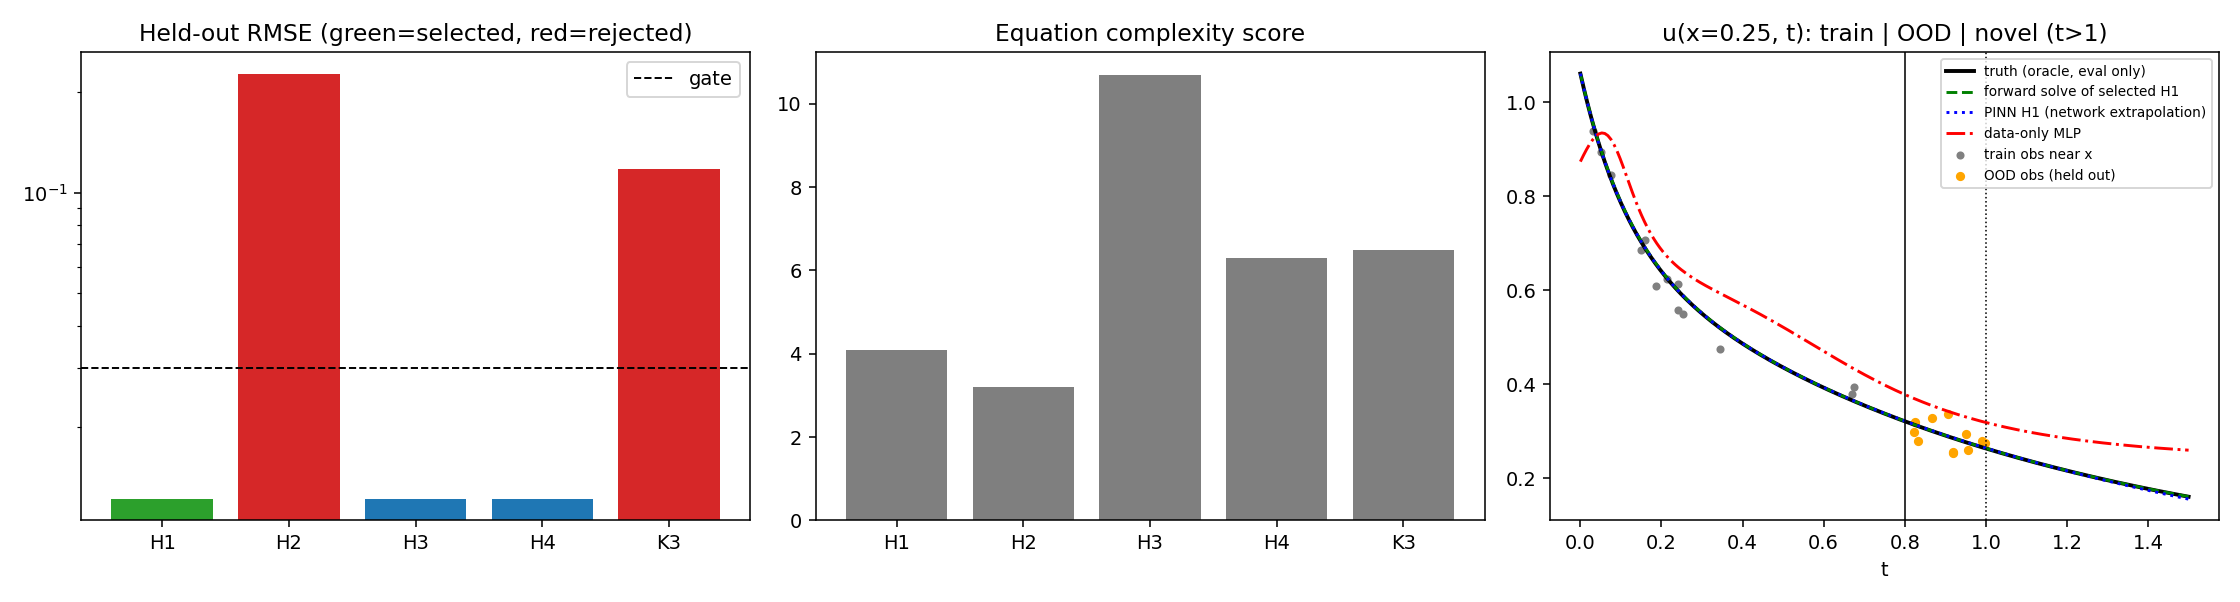
\includegraphics[width=\textwidth]{results/phase6/phase6_summary.png}
\caption{Phase~6 summary (from \fn{results/phase6/}): held-out error per candidate with the gate line (left),
complexity scores (middle), and a time trace at $x=0.25$ through train, OOD and novel windows (right).}
\end{figure}

\begin{caution}[: a disagreement reported, not hidden]
The bootstrap stability check (\fn{bootstrap_stability}) refits terms by least squares on finite-difference
derivatives, a cheap proxy, not PINN retraining and not Bayesian. For H3 it finds sign-stable $u$ and $u^2$
coefficients, while the PINN finds the reaction term contributes under 1\%. The same spurious terms appear in
Phase~2's noisy SINDy failure, which points to a finite-difference artefact. The report flags this instead of
choosing the convenient answer.
\end{caution}

% =====================================================================
\section{Phase 7: evaluation, attacks and generalisation}\label{sec:p7}
% =====================================================================

\textbf{Goal.} One success on one system proves little. Phase~7 asks: does the pipeline work across mechanism
families? Can it be fooled? Which components actually matter? Does it generalise to a new system?

\textbf{What was built} (the \fn{evaluation/} package, no new architecture):
\begin{itemize}
  \item \fn{datasets.py}: \textbf{12 benchmark datasets}, 4 families $\times$ 3 parameter settings, using exact
        analytic solutions where they exist and RK4 otherwise.
  \item \fn{describe.py}: turns any dataset into the text query for RAG with one fixed template; a test checks it
        never names a mechanism.
  \item \fn{engine.py}: the Phase~6 pipeline with the PINN swapped for fast least squares on finite-difference
        derivatives, so 95 items run in about a minute. (The PINN version runs separately on a second system.)
  \item \fn{identify.py}, \fn{benchmark.py}, \fn{adversarial.py}, \fn{ablation.py}, \fn{leakage.py}.
\end{itemize}

\begin{figure}[!htb]
\centering
% flowchart 'p7' -- shared by project_guide.tex and submission_report.tex
\begin{tikzpicture}[node distance=3.2mm and 7mm]
  \node[fnw=cExp] (main) {09_evaluation.main};
  \node[fnw=cEval, below=of main] (ds) {benchmark_datasets\\{\normalfont\tiny 12 datasets, cached to .npz}};
  \node[fnw=cEval, right=of ds] (mk) {_diffusion, _advection\\_adv_diff, _reaction_diffusion};
  \node[fnw=cEval, below=of ds] (res) {Resources\\{\normalfont\tiny corpus + RAG index + graph, built once}};
  \node[fnw=cEval, below=7mm of res] (bp) {build_pool};
  \node[fnw=cEval, right=of bp] (dsc) {describe_observations\\{\normalfont\tiny observation_stats $\to$ text}};
  \node[fnw=cEval, below=of dsc] (ctx) {build_scientific_context\\+ evidence templates + mock LLM};
  \node[fnw=cEval, below=10mm of bp] (vs) {validate_and_select};
  \node[fnw=cEval, below=of ctx] (fit) {fit_candidate_on_grid\\{\normalfont\tiny OLS on grid_fields}};
  \node[fnw=cVal, below=of fit] (sm) {select_model\\{\normalfont\tiny + _grid_param_contributions}};
  \node[fnw=cEval, below=of vs, yshift=-9mm] (ood) {predict_ood\\{\normalfont\tiny solve_forward to $t=1.3$}};
  \node[fnw=cEval, below=of ood] (sc) {score_run\\{\normalfont\tiny family_of, parameter + OOD error}};
  \begin{scope}[on background layer]
    \node[pkgbox=cEval, fit=(bp)(dsc)(sm)(sc), label={[pkglabel=cEval]above right:shared engine, run per dataset}] (eng) {};
  \end{scope}
  % suites
  \node[fnw=cEval, below=8mm of sc, xshift=-26mm] (s1) {run_single_questions\\{\normalfont\tiny 50 questions}};
  \node[fnw=cEval, right=4mm of s1] (s2) {run_multihop\\{\normalfont\tiny 25 multi-hop chains}};
  \node[fnw=cEval, right=4mm of s2] (s3) {run_adversarial\\{\normalfont\tiny 20 attacks; find_leaks}};
  \node[fnw=cEval, below=of s1] (s4) {run_ablation\\{\normalfont\tiny 7 arms; _discovery_only}};
  \node[fnw=cEval, right=4mm of s4] (s5) {leakage_audit\\{\normalfont\tiny decision_functions}};
  \node[fnw=cEval, right=4mm of s5] (s6) {real_llm + report\\{\normalfont\tiny phase7_report.md}};
  \draw[flow] (main) -- (ds); \draw[flow] (ds) -- (mk); \draw[flow] (ds) -- (res); \draw[flow] (res) -- (bp);
  \draw[flow] (bp) -- (dsc); \draw[flow] (dsc) -- (ctx); \draw[flow] (ctx) -- (bp.south east);
  \draw[flow] (bp) -- (vs); \draw[flow] (vs) -- (fit.west); \draw[flow] (fit) -- (sm); \draw[flow] (sm.west) -- (vs.south east);
  \draw[flow] (vs) -- (ood); \draw[flow] (ood) -- (sc);
  \draw[dflow] (s1.north) -- (s1.north |- eng.south);
  \draw[dflow] (s2.north) -- (s2.north |- eng.south);
  \draw[dflow] (s3.north) -- (s3.north |- eng.south);
\end{tikzpicture}

\pkglegend
\caption{Phase~7 function flow. A shared engine (shaded box) runs the pipeline on each benchmark dataset; the six
suites (bottom) call it in different ways. \fn{10_generalization.py} separately runs the full PINN pipeline
(\fn{validate_candidate}, \fn{select_model}) on a new system.}
\label{fig:p7}
\end{figure}

\subsection*{Results}

\textbf{50 questions: 50/50.} Structure identification 12/12, parameters within 5\% 12/12, plus graph, compiler,
complexity and retrieval-recall questions. Caveat: several categories are easy by construction, and
\textbf{top-1 retrieval is right only 1 time in 6}.

\textbf{25 multi-hop problems: 23/25.} The longest chains (data $\to$ description $\to$ RAG $\to$ graph $\to$
validation $\to$ selection $\to$ beyond-window prediction, 6 hops) score 12/12. Both failures come from top-1
lexical retrieval choosing ``advection'' for combined mechanisms.

\textbf{20 adversarial attacks: 20/20.} Examples: undeclared symbols, missing time derivative, negative
diffusivity, \emph{time-reversed data whose best fit needs $D<0$} (rejected by the physical bound), disguised
duplicates, malicious LLM output, the eigenfunction trap (flagged non-identifiable), a simpler-but-wrong
candidate on reaction--diffusion data (rejected at 85\% error rather than chosen for simplicity), corpus answer
leakage and prompt injection. Three noise/sparsity cases pass \emph{by abstention}: no candidate clears the gate,
which is safe but is not discovery.

\textbf{Ablation: which components matter?} (correct model out of 12 datasets)
\begin{center}
\small
\begin{tabular}{@{}lc@{}}
\toprule
\textbf{Arm} & \textbf{Correct} \\ \midrule
SINDy alone & 8/12 (advection--diffusion 0/3) \\
RAG + generation, no validation & 3/12 (always ``diffusion'') \\
RAG + graph + generation, no validation & 3/12 \\
\textbf{Full system} & \textbf{12/12} \\
Full system with the original Phase~6 rule & 10/12 \\
Full system without the LLM & 12/12 \\
Retrieved-evidence equations + validation (no graph, no LLM) & 12/12 \\
\bottomrule
\end{tabular}
\end{center}

\begin{lesson}[: what each part really contributes]
Physics validation and selection produce the correct answers; without them, generation just repeats its
favourite guess. RAG supplies a candidate pool that contains the truth. On this benchmark, the graph and the
\emph{mock} LLM add no measurable accuracy; the graph's value is structured querying and provenance. SINDy is
fast and accurate when every true term is large, but its threshold silently drops small real terms. And
\textbf{accurate prediction is not the same as the right law}: the Phase~6 rule predicted OOD well on 12/12 while
identifying only 10/12 laws correctly.
\end{lesson}

\textbf{The disclosed rule change.} On noise-free two-mode diffusion, finite-difference $u_{xx}$ gives each sine
mode a slightly wrong decay rate, and the extra $u$ term of reaction--diffusion corrects both modes exactly, so
that model fits the \emph{discretisation error} to $10^{-14}$ and wins ``within 5\% of best''. Yet its reaction
term contributes only 0.27\% of the dynamics. Phase~7 therefore promoted term necessity into the rule (the
``inactive?'' step in Figure~\ref{fig:selection}), as an opt-in flag so Phase~6 results stay reproducible. It
changes 2 of 12 benchmark outcomes and never strips a real reaction term.

\textbf{Generalisation to a new system with the full PINN pipeline.} Hidden truth:
$u_t + 0.4\,u_x = 0.02\,u_{xx}$ on $x\in[0,1.5]$, Gaussian start, 400 points with 5\% noise.
\begin{center}
\footnotesize\setlength{\tabcolsep}{4pt}
\begin{tabular}{@{}lllll@{}}
\toprule
\textbf{Candidate} & \textbf{Fitted} & \textbf{Holdout RMSE} & \textbf{Status} & \textbf{OOD vs clean (oracle)} \\ \midrule
diffusion & $D=0.075$ & 0.096 & rejected & 0.111 \\
advection & $c=0.369$ & 0.064 & rejected & 0.113 \\
reaction--diffusion & $D=0.117,\ r=1.22,\ K=1.44$ & 0.084 & rejected & 0.095 \\
\textbf{advection--diffusion} & $c=0.39897,\ D=0.02008$ & \textbf{0.0099} & \textbf{selected} & \textbf{0.0010} \\
data-only MLP & -- & 0.0124 & -- & 0.0068 \\
\bottomrule
\end{tabular}
\end{center}
Both constants within 0.4\% of the truth; solving the law forward beyond the data gives 0.58\% relative error.
SINDy on the same noisy data returned a spurious equation.

\textbf{Leakage audit.} A static code check confirms none of the six decision functions reference ground-truth
names; none of the 15 hidden benchmark values appears in the corpus; and the audit catches a deliberately planted
cheating selector, so the check is not vacuous.
